% Options for packages loaded elsewhere
\PassOptionsToPackage{unicode}{hyperref}
\PassOptionsToPackage{hyphens}{url}
%
\documentclass[
]{article}
\usepackage{amsmath,amssymb}
\usepackage{lmodern}
\usepackage{ifxetex,ifluatex}
\ifnum 0\ifxetex 1\fi\ifluatex 1\fi=0 % if pdftex
  \usepackage[T1]{fontenc}
  \usepackage[utf8]{inputenc}
  \usepackage{textcomp} % provide euro and other symbols
\else % if luatex or xetex
  \usepackage{unicode-math}
  \defaultfontfeatures{Scale=MatchLowercase}
  \defaultfontfeatures[\rmfamily]{Ligatures=TeX,Scale=1}
  \setmainfont[]{CMU Serif}
\fi
% Use upquote if available, for straight quotes in verbatim environments
\IfFileExists{upquote.sty}{\usepackage{upquote}}{}
\IfFileExists{microtype.sty}{% use microtype if available
  \usepackage[]{microtype}
  \UseMicrotypeSet[protrusion]{basicmath} % disable protrusion for tt fonts
}{}
\makeatletter
\@ifundefined{KOMAClassName}{% if non-KOMA class
  \IfFileExists{parskip.sty}{%
    \usepackage{parskip}
  }{% else
    \setlength{\parindent}{0pt}
    \setlength{\parskip}{6pt plus 2pt minus 1pt}}
}{% if KOMA class
  \KOMAoptions{parskip=half}}
\makeatother
\usepackage{xcolor}
\IfFileExists{xurl.sty}{\usepackage{xurl}}{} % add URL line breaks if available
\IfFileExists{bookmark.sty}{\usepackage{bookmark}}{\usepackage{hyperref}}
\hypersetup{
  pdftitle={Введение в иерархический кластерный анализ: матрица расстояний, метод агломерации, дендрограмма},
  pdfauthor={Алла Тамбовцева},
  hidelinks,
  pdfcreator={LaTeX via pandoc}}
\urlstyle{same} % disable monospaced font for URLs
\usepackage[margin=1in]{geometry}
\usepackage{color}
\usepackage{fancyvrb}
\newcommand{\VerbBar}{|}
\newcommand{\VERB}{\Verb[commandchars=\\\{\}]}
\DefineVerbatimEnvironment{Highlighting}{Verbatim}{commandchars=\\\{\}}
% Add ',fontsize=\small' for more characters per line
\usepackage{framed}
\definecolor{shadecolor}{RGB}{248,248,248}
\newenvironment{Shaded}{\begin{snugshade}}{\end{snugshade}}
\newcommand{\AlertTok}[1]{\textcolor[rgb]{0.94,0.16,0.16}{#1}}
\newcommand{\AnnotationTok}[1]{\textcolor[rgb]{0.56,0.35,0.01}{\textbf{\textit{#1}}}}
\newcommand{\AttributeTok}[1]{\textcolor[rgb]{0.77,0.63,0.00}{#1}}
\newcommand{\BaseNTok}[1]{\textcolor[rgb]{0.00,0.00,0.81}{#1}}
\newcommand{\BuiltInTok}[1]{#1}
\newcommand{\CharTok}[1]{\textcolor[rgb]{0.31,0.60,0.02}{#1}}
\newcommand{\CommentTok}[1]{\textcolor[rgb]{0.56,0.35,0.01}{\textit{#1}}}
\newcommand{\CommentVarTok}[1]{\textcolor[rgb]{0.56,0.35,0.01}{\textbf{\textit{#1}}}}
\newcommand{\ConstantTok}[1]{\textcolor[rgb]{0.00,0.00,0.00}{#1}}
\newcommand{\ControlFlowTok}[1]{\textcolor[rgb]{0.13,0.29,0.53}{\textbf{#1}}}
\newcommand{\DataTypeTok}[1]{\textcolor[rgb]{0.13,0.29,0.53}{#1}}
\newcommand{\DecValTok}[1]{\textcolor[rgb]{0.00,0.00,0.81}{#1}}
\newcommand{\DocumentationTok}[1]{\textcolor[rgb]{0.56,0.35,0.01}{\textbf{\textit{#1}}}}
\newcommand{\ErrorTok}[1]{\textcolor[rgb]{0.64,0.00,0.00}{\textbf{#1}}}
\newcommand{\ExtensionTok}[1]{#1}
\newcommand{\FloatTok}[1]{\textcolor[rgb]{0.00,0.00,0.81}{#1}}
\newcommand{\FunctionTok}[1]{\textcolor[rgb]{0.00,0.00,0.00}{#1}}
\newcommand{\ImportTok}[1]{#1}
\newcommand{\InformationTok}[1]{\textcolor[rgb]{0.56,0.35,0.01}{\textbf{\textit{#1}}}}
\newcommand{\KeywordTok}[1]{\textcolor[rgb]{0.13,0.29,0.53}{\textbf{#1}}}
\newcommand{\NormalTok}[1]{#1}
\newcommand{\OperatorTok}[1]{\textcolor[rgb]{0.81,0.36,0.00}{\textbf{#1}}}
\newcommand{\OtherTok}[1]{\textcolor[rgb]{0.56,0.35,0.01}{#1}}
\newcommand{\PreprocessorTok}[1]{\textcolor[rgb]{0.56,0.35,0.01}{\textit{#1}}}
\newcommand{\RegionMarkerTok}[1]{#1}
\newcommand{\SpecialCharTok}[1]{\textcolor[rgb]{0.00,0.00,0.00}{#1}}
\newcommand{\SpecialStringTok}[1]{\textcolor[rgb]{0.31,0.60,0.02}{#1}}
\newcommand{\StringTok}[1]{\textcolor[rgb]{0.31,0.60,0.02}{#1}}
\newcommand{\VariableTok}[1]{\textcolor[rgb]{0.00,0.00,0.00}{#1}}
\newcommand{\VerbatimStringTok}[1]{\textcolor[rgb]{0.31,0.60,0.02}{#1}}
\newcommand{\WarningTok}[1]{\textcolor[rgb]{0.56,0.35,0.01}{\textbf{\textit{#1}}}}
\usepackage{graphicx}
\makeatletter
\def\maxwidth{\ifdim\Gin@nat@width>\linewidth\linewidth\else\Gin@nat@width\fi}
\def\maxheight{\ifdim\Gin@nat@height>\textheight\textheight\else\Gin@nat@height\fi}
\makeatother
% Scale images if necessary, so that they will not overflow the page
% margins by default, and it is still possible to overwrite the defaults
% using explicit options in \includegraphics[width, height, ...]{}
\setkeys{Gin}{width=\maxwidth,height=\maxheight,keepaspectratio}
% Set default figure placement to htbp
\makeatletter
\def\fps@figure{htbp}
\makeatother
\setlength{\emergencystretch}{3em} % prevent overfull lines
\providecommand{\tightlist}{%
  \setlength{\itemsep}{0pt}\setlength{\parskip}{0pt}}
\setcounter{secnumdepth}{-\maxdimen} % remove section numbering
\usepackage[russian]{babel}
\usepackage{hyperref}
\hypersetup{colorlinks = true, urlcolor = blue, linkcolor=blue}
\ifluatex
  \usepackage{selnolig}  % disable illegal ligatures
\fi

\title{Введение в иерархический кластерный анализ: матрица расстояний,
метод агломерации, дендрограмма}
\author{Алла Тамбовцева}
\date{}

\begin{document}
\maketitle

\large

Реализуем в R иерархический кластерный анализ, который мы проделали на
семинаре вручную. У нас есть четыре наблюдения и две переменные, \(X\) и
\(Y\). Запишем значения в векторы, а затем объединим их в датафрейм:

\begin{Shaded}
\begin{Highlighting}[]
\NormalTok{x }\OtherTok{\textless{}{-}} \FunctionTok{c}\NormalTok{(}\DecValTok{0}\NormalTok{, }\DecValTok{7}\NormalTok{, }\DecValTok{1}\NormalTok{, }\DecValTok{4}\NormalTok{)}
\NormalTok{y }\OtherTok{\textless{}{-}} \FunctionTok{c}\NormalTok{(}\DecValTok{4}\NormalTok{, }\DecValTok{0}\NormalTok{, }\DecValTok{2}\NormalTok{, }\DecValTok{2}\NormalTok{)}

\NormalTok{dat }\OtherTok{\textless{}{-}} \FunctionTok{cbind.data.frame}\NormalTok{(x, y)}
\NormalTok{dat}
\end{Highlighting}
\end{Shaded}

\begin{verbatim}
##   x y
## 1 0 4
## 2 7 0
## 3 1 2
## 4 4 2
\end{verbatim}

\textbf{Примечание 1:} \texttt{cbind} соответствует объединению по
столбцам (от \emph{columns}), \texttt{rbind} --- объединению по строкам
(от \emph{rows}).

\textbf{Примечание 2:} в данном случае функция \texttt{cbind()} тоже бы
подошла, только стоит иметь в виду, что она создаёт матрицу, а не
датафрейм. Проблема может возникнуть тогда, когда \texttt{x} и
\texttt{y} являются векторами разного типа, при объединении в матрицу
все элементы будут приведены к одному типу. Победит более сильный тип:
например, строковый (\emph{character}) вытеснит числовой
(\emph{numeric}), и все элементы станут текстовыми.

Построим матрицу расстояний \texttt{D}, но прежде шкалируем наши данные
с помощью функции \texttt{scale()}: вычтем из каждого значения в столбце
\texttt{x} среднее по столбцу и поделим на стандартное отклонение по
столбцу, затем проделаем то же самое для столбца \texttt{y}:

\begin{Shaded}
\begin{Highlighting}[]
\FunctionTok{dist}\NormalTok{(}\FunctionTok{scale}\NormalTok{(dat))}
\end{Highlighting}
\end{Shaded}

\begin{verbatim}
##           1         2         3
## 2 3.3015148                    
## 3 1.2649111 2.2583180          
## 4 1.7606817 1.5491933 0.9486833
\end{verbatim}

Матрица в R получилась довольно экономной: она показывает только
расстояния между различными точками и не дублирует одни и те же
расстояния, предполагая, что матрица симметричная. По умолчанию функция
\texttt{dist()} считает евклидово расстояние. Запросим документацию
функции через \texttt{?}:

\begin{Shaded}
\begin{Highlighting}[]
\NormalTok{?dist}
\end{Highlighting}
\end{Shaded}

Список доступных расстояний:

\begin{itemize}
\tightlist
\item
  \texttt{euclidean}: евклидово расстояние;
\item
  \texttt{maximum}: расстояние Чебышёва;
\item
  \texttt{manhattan}: манхэттенское расстояние;
\item
  \texttt{canberra}:
  \href{https://en.wikipedia.org/wiki/Canberra_distance}{канберрское}
  расстояние;
\item
  \texttt{binary}: асимметричное бинарное расстояние;
\item
  \texttt{minkowski}: расстояние
  \href{https://en.wikipedia.org/wiki/Minkowski_distance}{Минковского}.
\end{itemize}

Вычислим манхэттенское расстояние (оно было нужно нам по условию) и
сохраним матрицу расстояний в переменную \texttt{D}:

\begin{Shaded}
\begin{Highlighting}[]
\NormalTok{D }\OtherTok{\textless{}{-}} \FunctionTok{dist}\NormalTok{(}\FunctionTok{scale}\NormalTok{(dat), }\AttributeTok{method =} \StringTok{"manhattan"}\NormalTok{)}
\NormalTok{D}
\end{Highlighting}
\end{Shaded}

\begin{verbatim}
##           1         2         3
## 2 4.6630841                    
## 3 1.5409726 3.1221115          
## 4 2.4896559 2.1734282 0.9486833
\end{verbatim}

Теперь запустим иерархический кластерный анализ, выберем метод дальнего
соседа, метод полной связи (\texttt{complete}):

\begin{Shaded}
\begin{Highlighting}[]
\NormalTok{hc }\OtherTok{\textless{}{-}} \FunctionTok{hclust}\NormalTok{(D, }\AttributeTok{method =} \StringTok{"complete"}\NormalTok{)}
\NormalTok{hc}
\end{Highlighting}
\end{Shaded}

\begin{verbatim}
## 
## Call:
## hclust(d = D, method = "complete")
## 
## Cluster method   : complete 
## Distance         : manhattan 
## Number of objects: 4
\end{verbatim}

По умолчанию функция \texttt{hclust()} использует именно этот метод,
поэтому в данном случае аргумент \texttt{method} можно было бы опустить.
Список основных методов такой:

\begin{itemize}
\tightlist
\item
  \texttt{complete}: метод полной связи;
\item
  \texttt{single}: метод одиночной связи;
\item
  \texttt{average}: метод средней связи;
\item
  \texttt{median}: метод медианной связи;
\item
  \texttt{centroid}: метод центроидной связи.
\end{itemize}

Осталось только построить дендрограмму, для этого потребуется базовая
функция \texttt{plot()}:

\begin{Shaded}
\begin{Highlighting}[]
\FunctionTok{plot}\NormalTok{(hc, }\AttributeTok{main =} \StringTok{"Complete linkage method"}\NormalTok{)}
\end{Highlighting}
\end{Shaded}

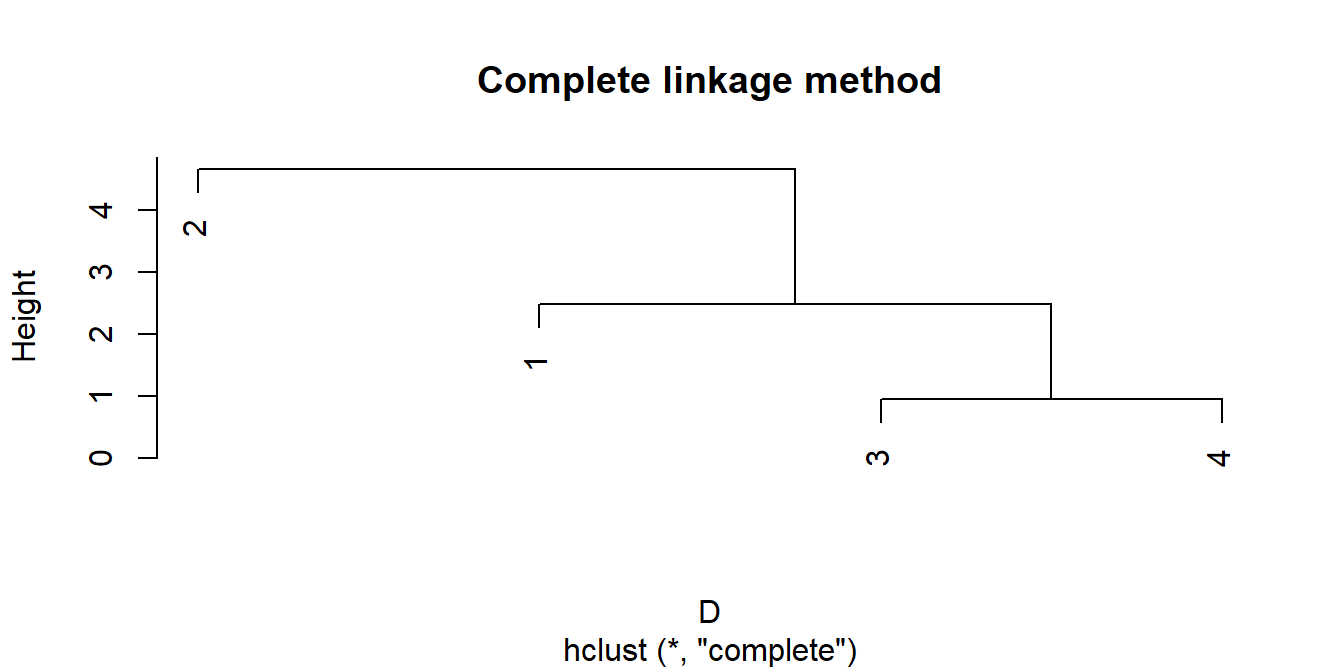
\includegraphics{CLUSTER01_files/figure-latex/unnamed-chunk-6-1.pdf}

Если мы определились с числом кластеров, можем выделить их на
дендрограмме явно, с помощью прямоугольников:

\begin{Shaded}
\begin{Highlighting}[]
\FunctionTok{plot}\NormalTok{(hc, }\AttributeTok{main =} \StringTok{"Complete linkage method"}\NormalTok{)}
\FunctionTok{rect.hclust}\NormalTok{(hc, }\AttributeTok{k =} \DecValTok{2}\NormalTok{, }\AttributeTok{border =} \StringTok{"red"}\NormalTok{)}
\end{Highlighting}
\end{Shaded}

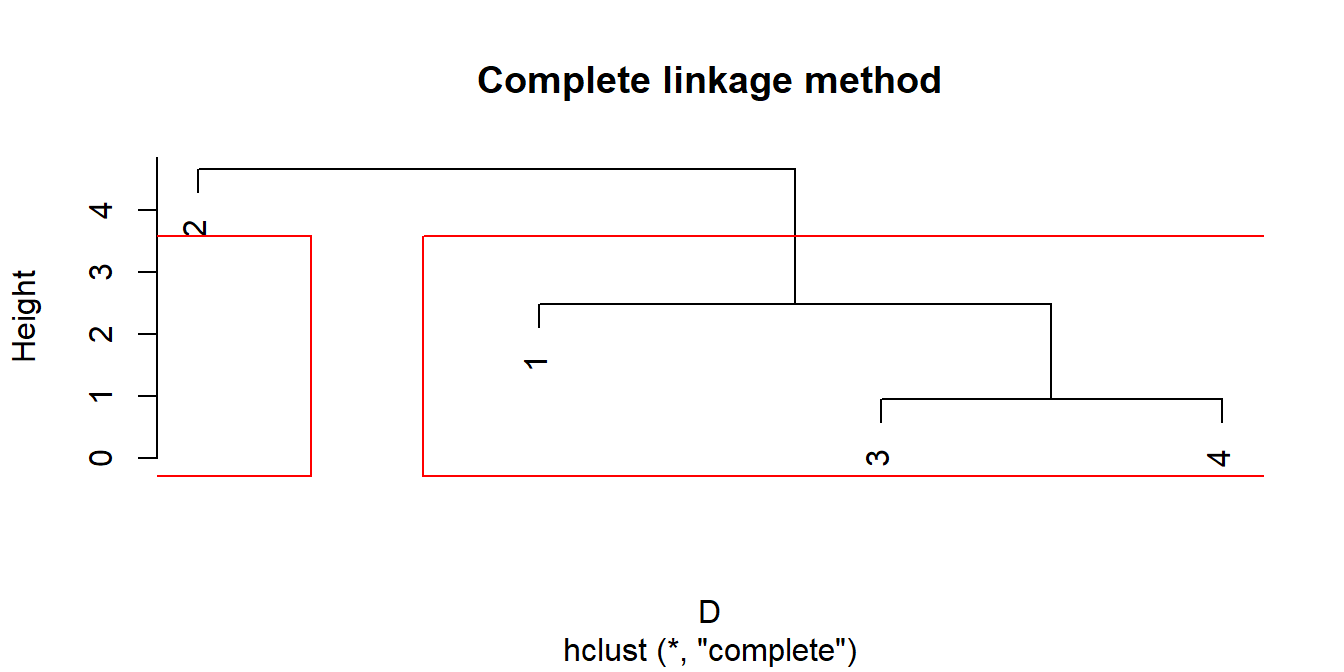
\includegraphics{CLUSTER01_files/figure-latex/unnamed-chunk-7-1.pdf}

\textbf{Примечание:} функция \texttt{rect.hclust()} добавляет
прямоугольники на уже существующий график, то есть накладывает ещё один
слой c графическими элементами. Поэтому эта строка с кодом должна
запускаться сразу после \texttt{plot()}. Если запустить её два раза с
разным \texttt{k}, не перезапустив строку с \texttt{plot()},
прямоугольники тоже добавятся два раза, поэтому не забывайте обновлять
саму дендрограмму.

Из объекта \texttt{hc}, который нам создала функция \texttt{hclust()},
можно извлекать отдельные элементы. Например, расстояния, при которых
производилось объединение кластеров на каждой итерации алгоритма:

\begin{Shaded}
\begin{Highlighting}[]
\NormalTok{hc}\SpecialCharTok{$}\NormalTok{height}
\end{Highlighting}
\end{Shaded}

\begin{verbatim}
## [1] 0.9486833 2.4896559 4.6630841
\end{verbatim}

Или метки наблюдений в том порядке, в котором они упорядочены на
дендрограмме:

\begin{Shaded}
\begin{Highlighting}[]
\NormalTok{hc}\SpecialCharTok{$}\NormalTok{order}
\end{Highlighting}
\end{Shaded}

\begin{verbatim}
## [1] 2 1 3 4
\end{verbatim}

А ещё меткам можно присвоить свои обозначения, если текущие нас не
устраивают. Создадим вектор, состоящий из букв A, B, C, D:

\begin{Shaded}
\begin{Highlighting}[]
\NormalTok{labs }\OtherTok{\textless{}{-}}\NormalTok{ LETTERS[}\DecValTok{1}\SpecialCharTok{:}\DecValTok{4}\NormalTok{]}
\NormalTok{labs}
\end{Highlighting}
\end{Shaded}

\begin{verbatim}
## [1] "A" "B" "C" "D"
\end{verbatim}

\textbf{Примечание:} \texttt{LETTERS} --- встроенный вектор из заглавных
букв английского алфавита, выбираем первые четыре. Есть ещё вектор
\texttt{letters} (строчные буквы английского алфавита),
\texttt{month.name} (названия месяцев на английском) и
\texttt{month.abb} (сокращённые названия месяцев на английском).

Запишем новые метки в \texttt{hc}:

\begin{Shaded}
\begin{Highlighting}[]
\NormalTok{hc}\SpecialCharTok{$}\NormalTok{labels }\OtherTok{\textless{}{-}}\NormalTok{ labs}
\end{Highlighting}
\end{Shaded}

И построим дендрограмму по \texttt{hc} ещё раз:

\begin{Shaded}
\begin{Highlighting}[]
\FunctionTok{plot}\NormalTok{(hc, }\AttributeTok{main =} \StringTok{"Complete linkage method"}\NormalTok{)}
\end{Highlighting}
\end{Shaded}

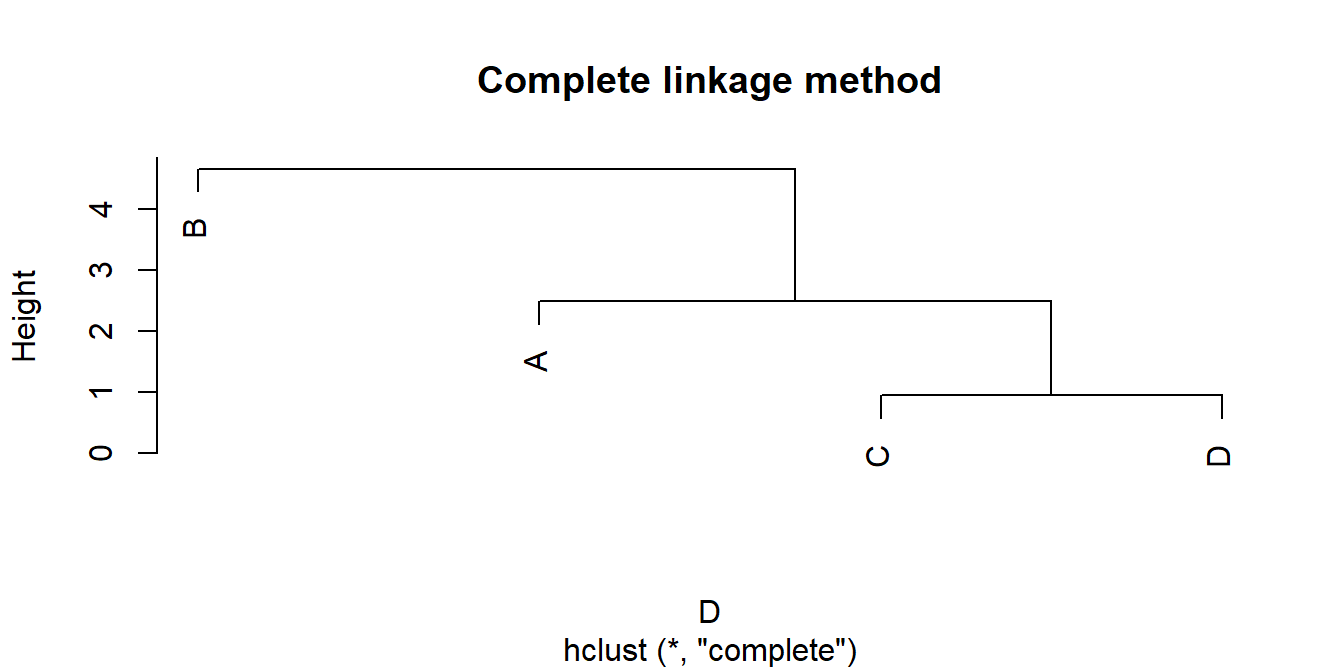
\includegraphics{CLUSTER01_files/figure-latex/unnamed-chunk-12-1.pdf}

\end{document}
